\section{Results}

We ran the calculation for all the adaptivity types 
in both single-mesh and multi-mesh configurations. The following results
were recorded: converged error at each time step, cumulative CPU
time at each time step, and the problem size in terms of number
of degrees of freedoms (NDOFs) at each time step.  
Two types of initial meshes were used --- in case of only \emph{p}-adaptivity,
more refined mesh was used. When also the element size refinement
was enabled (all \emph{h} adaptivity types), very coarse initial mesh
was used. In any case, the initial mesh was loaded at each time step.

Some initial observations
helped to select the graphs for this work --- it would have been unreasonable 
to present all recorded results for each adaptivity type.
First of all, the multi-mesh configuration resulted smaller problem size, faster
calculation, and better or similar error convergence than the single-mesh
configuration for all but HP\_ANISO\_H adaptivity type. In this case
the single-mesh configuration resulted slightly but not significantly
smaller problem size. It must be also noted that in case of isotropic
refinements, only P\_ISO resulted in a reasonable problem size.
Secondly, H\_ISO did not converge very well in terms of the
calculation time and the problem size. The term ``reasonable problem size''
means that the number of degrees of freedom in time converges
to so that $N_{dof}<500$, and the term ``reasonable calculation time''
means that the calculation (step $\tau=0.01\ s$, physical
time $t_{end}=3.0\ s$) time $t$ on a givem system was $t<500\ s$.
Although these parameters are empirical, they are reasonable given
that the most adaptivity modes gave significantly smaller results,
e.g. $t<<500\ s$ and $N_{dof} << 500$.
Therefore the multi-mesh calculation results H\_ISO, H\_ANSIO, P\_ANISO,
HP\_ANISO, HP\_ANISO\_P and the single-mesh calculation results of HP\_ANISO\_H
adaptivity mode are compared. In all cases, the error at each time step remained below
the threshold which were set to $e_{th}=0.5\%$ between the coarse mesh
and fine mesh solutions.

\begin{figure}
  \begin{centering}
  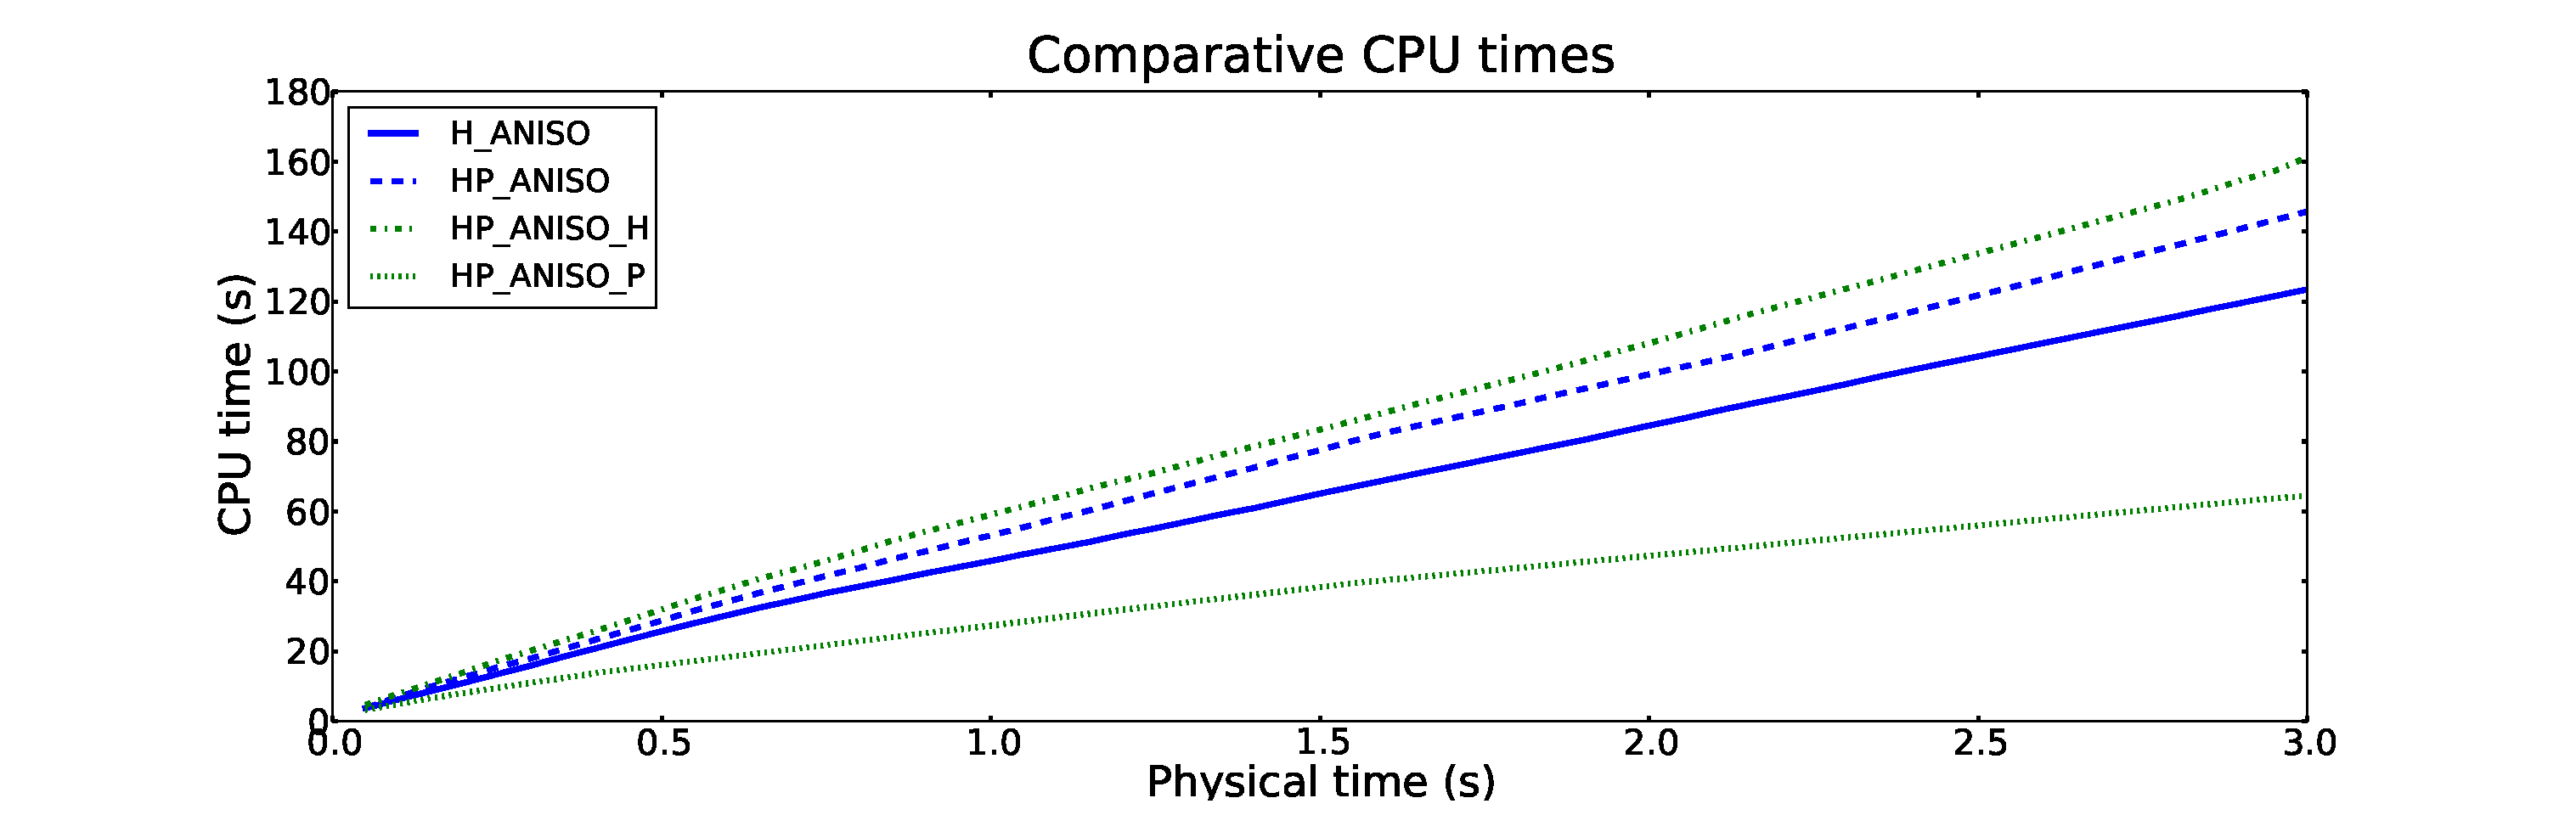
\includegraphics[width=\columnwidth]{cpu}
  \caption{\label{fig:cpu} Cumulative CPU time for different adaptivity modes.}
  \end{centering}
\end{figure}

\begin{figure}
  \begin{centering}
  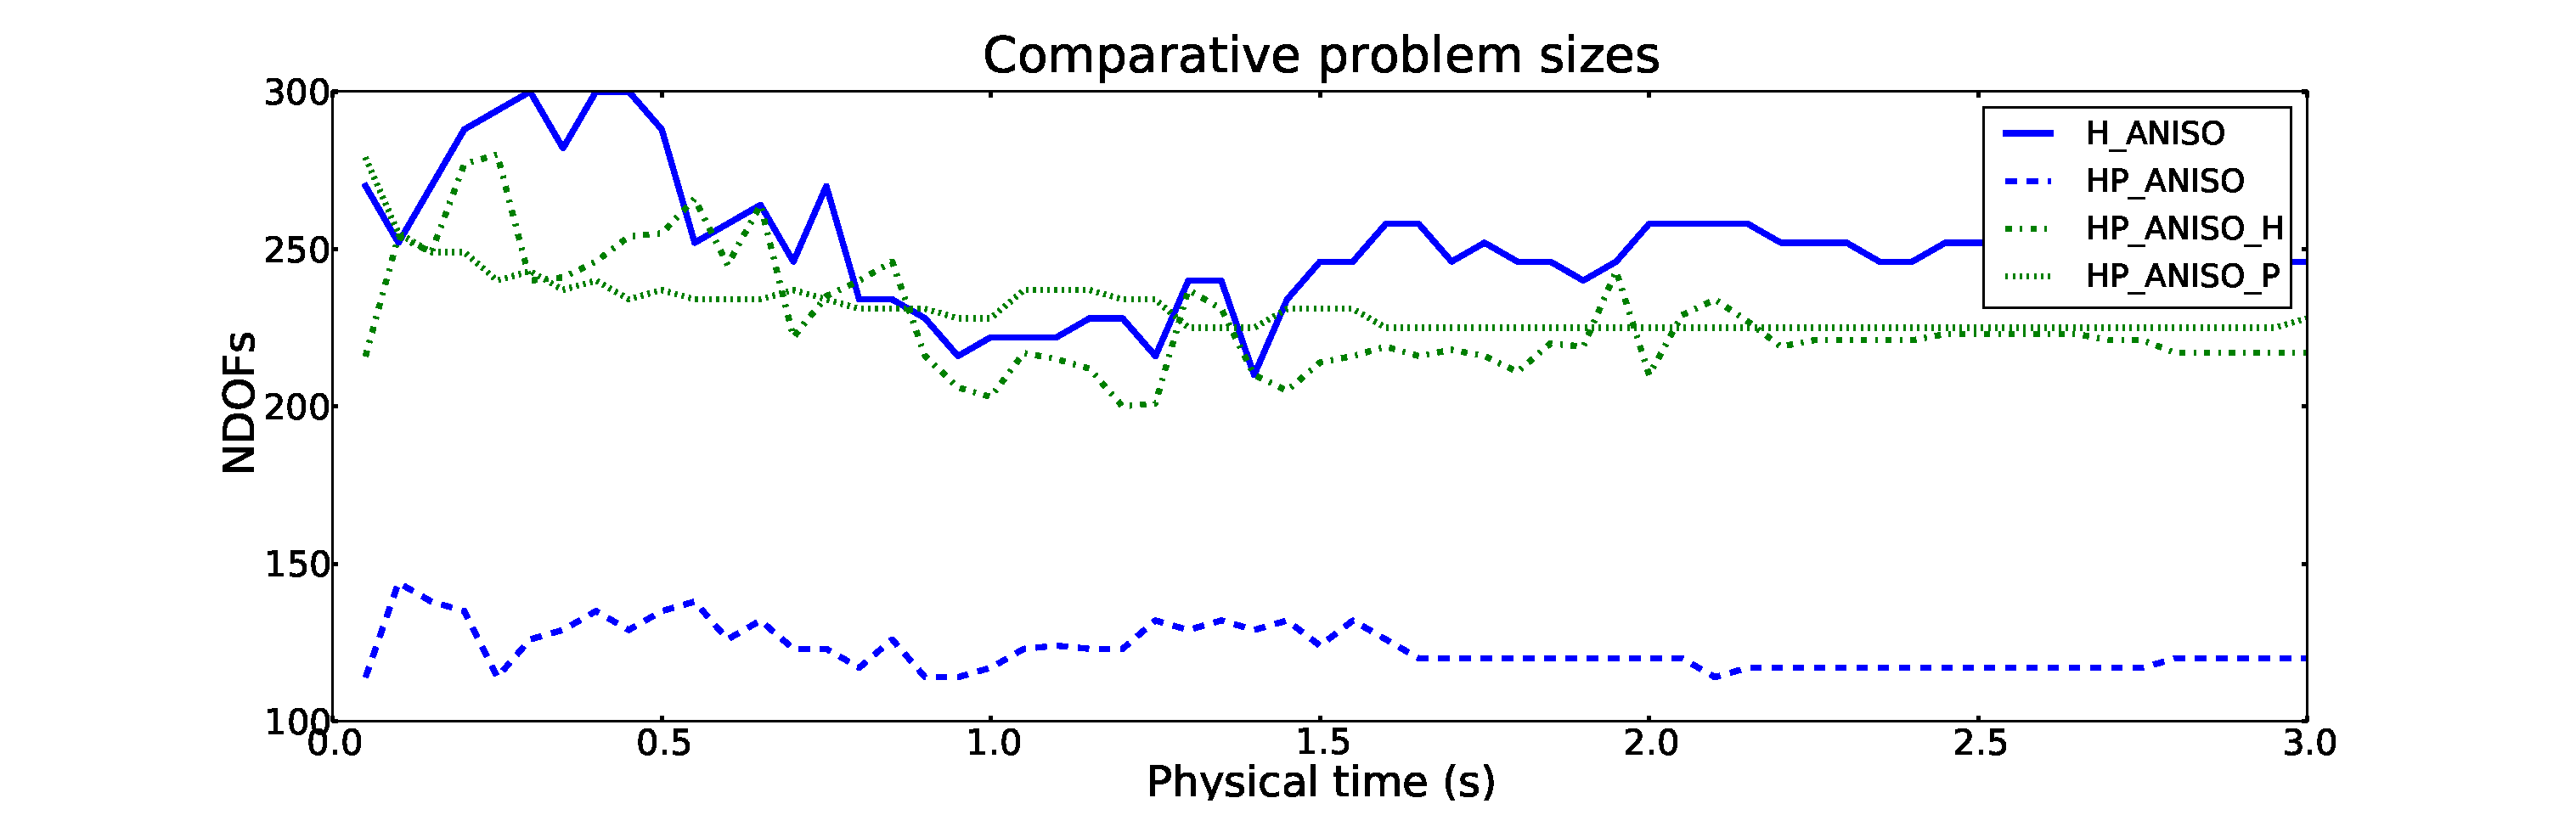
\includegraphics[width=\columnwidth]{dof}
  \caption{\label{fig:dof} NDOFs at each time step for different adaptivity modes.}
  \end{centering}
\end{figure}

Fig.~\ref{fig:cpu} shows the cumulative CPU time for different adaptivity
modes at each time step. All the calculations were done on the same computer
at similar conditions. Here we see that HP\_ANISO takes the most
resources, which is also expected as this adaptivity mode contains the most
candidates (see XXX) from which the refinement methode is chosen from.
At the same time, HP\_ANISO\_H is the fastest.
Fig.~\ref{fig:dof} shows the NDOFs at each time step for different adaptivity modes.
There we see that the HP\_ANISO results in the smallest problem size. All other
adaptivity modes result in a similar problem size ($N_{dof} \approx 250$), however,
\emph{p}-adaptivity modes P\_ISO and P\_ANISO start off with relatively large $N_{dof}$.



TODO, some conclusions TODO

a) HP\_ANISO is the best in terms of problem size

b) P\_ANISO and P\_ISO are good during most part of the problem, however,
initial time step would benefit from the h adaptivity

c) P\_ISO and HP\_ANISO\_H and HP\_ANISO\_P are the fastest, but here
we have to consider, that P\_ISO starts off from more refined mesh.

